\documentclass[a4paper]{article}

\usepackage[english]{babel}
\usepackage[utf8]{inputenc}
\usepackage{amsmath}
\usepackage{graphicx}
\usepackage[firstpage]{draftwatermark}
\SetWatermarkScale{5}
\SetWatermarkLightness{0.8}
\SetWatermarkText{DRAFT}


\usepackage{xargs}                      % Use more than one optional parameter in a new commands
\usepackage[pdftex,dvipsnames]{xcolor}  % Coloured text etc.

\usepackage[colorinlistoftodos,prependcaption,textsize=small]{todonotes}

% redefinition of todo
\newcommandx{\rtealgo}[2][1=]{\todo[linecolor=orange,backgroundcolor=orange!25,bordercolor=orange,#1]{#2}}
\newcommandx{\unsure}[2][1=]{\todo[linecolor=red,backgroundcolor=red!25,bordercolor=red,#1]{#2}}
\newcommandx{\atmosconfig}[2][1=]{\todo[linecolor=blue,backgroundcolor=blue!25,bordercolor=blue,#1]{#2}}
\newcommandx{\molscatprocess}[2][1=]{\todo[linecolor=red,backgroundcolor=red!25,bordercolor=red,#1]{#2}}
\newcommandx{\molabsprocess}[2][1=]{\todo[linecolor=green,backgroundcolor=green!25,bordercolor=green,#1]{#2}}
\newcommandx{\molabsmodel}[2][1=]{\todo[linecolor=yellow,backgroundcolor=yellow!25,bordercolor=yellow,#1]{#2}}
\newcommandx{\molabscompo}[2][1=]{\todo[linecolor=Plum,backgroundcolor=Plum!25,bordercolor=Plum,#1]{#2}}
\newcommandx{\allruns}[2][1=]{\todo[linecolor=OliveGreen,backgroundcolor=OliveGreen!25,bordercolor=OliveGreen,#1]{#2}}
\newcommandx{\aerosols}[2][1=]{\todo[linecolor=gray,backgroundcolor=gray!25,bordercolor=gray,#1]{#2}}


\newcommandx{\thiswillnotshow}[2][1=]{\todo[disable,#1]{#2}}
%

\usepackage{hyperref}

\title{Prescriptions to generate Modtran and LibRadtran predictions for air transparency at LSST site}

\author{Sylvie Dagoret-Campagne, Kirk Gilmore}

\date{\today}

\begin{document}
\maketitle

\begin{abstract}
This note aims specifying a set of atmospheric configurations, in order to compare the air transparencies predictions  by Modtran and LibRadtran for LSST site.
Starting from similar atmospheric model, we want to check the level of agreement between both predictions within
the accuracies of LSST photometry as well as auxiliary telescope wavelength resolution. 
\end{abstract}

\section{Introduction}
%----------------------------
\label{sec:introduction}
We want to compare air-transparency predicted by Modtran and LibRadtran for LSST observatory site.
This comparison can be done only if we choose common configuration parameters for the kind of atmosphere  from which both simulators can calculate air attenuation.

\section{Common configuration parameters}
%--------------------------------------------------------


\subsection{Wavelength range and accuracy}
%---------------------------------------------------------

\todo[inline]{{\bf Wavelength :}  $\lambda \in [250,1200]$~nm, $\Delta \lambda=$1~nm}
It must be noticed that every light interaction process may not be defined over this whole range. For example, in LibRadtran, one cannot simulate with wavelength smaller than 250~nm, except for special cases. 

\subsection{LSST site}
%-----------------------------
\todo[inline]{{\bf Altitude :} $h=2.680$~km.}

\subsection{Zenith angle}
%---------------------------------
We want to compare the air shower simulator over a wide range of airmass values. Thus we recommends to  simulate air-transparencies for  
\todo[inline]{{\bf Airmass  :}  $z$ computed for 31 points in steps of 0.1~: $z \in [1,3]$.}
Usually, simulation programs need the zenith angle $\theta_{z}$ as input parameter.
Then we should use the simple relation between $\theta_{z}$ and $z$~:
\begin{equation}
z=\sec \theta_{z}=\frac{1}{\cos \theta_z}
\end{equation}



\section{Solvers and Geometry options}
%-------------------------------------------------

Because we want to compare calculations at high airmass, we have to compare calculations performed either under the standard parallel plane approximation and also under the pseudo-spherical correction.
The we recommends to select two Radiative Transfer Equation (RTE) solvers~:
\rtealgo[inline]{{\bf Two RTE solvers~:} "$disort$" for Parallel Plane approximation and "$sdisort$" for Pseudo-Spherical correction. } 


\section{Atmospheric models}
%-------------------------------------

There are several pre-defined atmospheres in both simulation packages. These atmospheres are defined by their
vertical profile of the Temperature, Pressure and Air densities. The typical profiles expected are shown on figure~\ref{fig:rt_atmprof}.

\begin{figure}
\centering
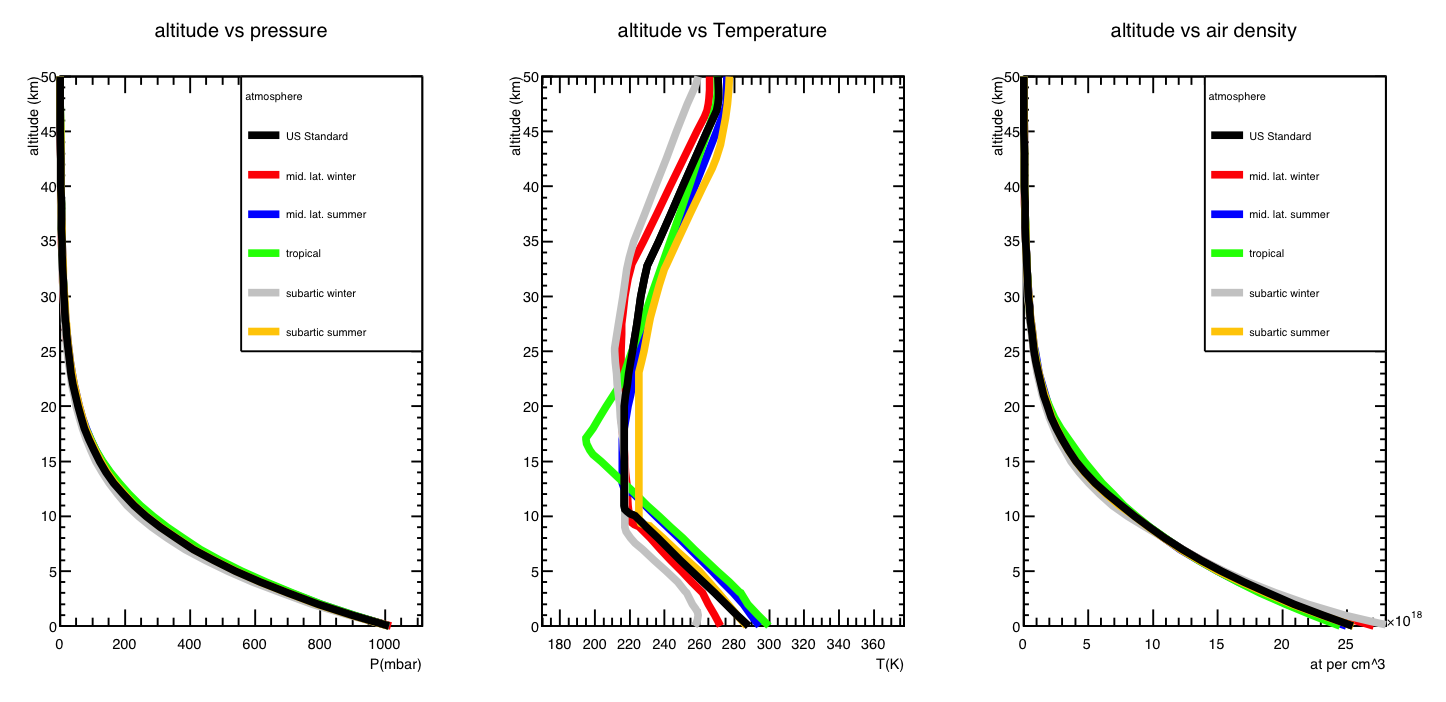
\includegraphics[width=1\textwidth]{images/rt_atmprof.png}
\caption{\label{fig:rt_atmprof}Vertical profiles for Temperature, Pressure and Air density for typical atmospheres in LibRadtran.}
\end{figure}
If pressure and air density may not vary a lot from one atmospheric model to another, Temperature profiles may be quite different, especially at ground and also at temperature inversion altitude at $h=15-20$~km.
We will see that Temperature has an impact on absorption coefficient but has little effect on scattering processes like Rayleigh and Aerosols.

Then looking at molecular species vertical profiles densities on figure~\ref{fig:rt_atm_densities}, we can notice the large dispersion between the various atmosphere on precipitable water level close to ground and also on ozone at $h=15-20$~km, precisely where Temperature has significant variations.
\begin{figure}
\centering
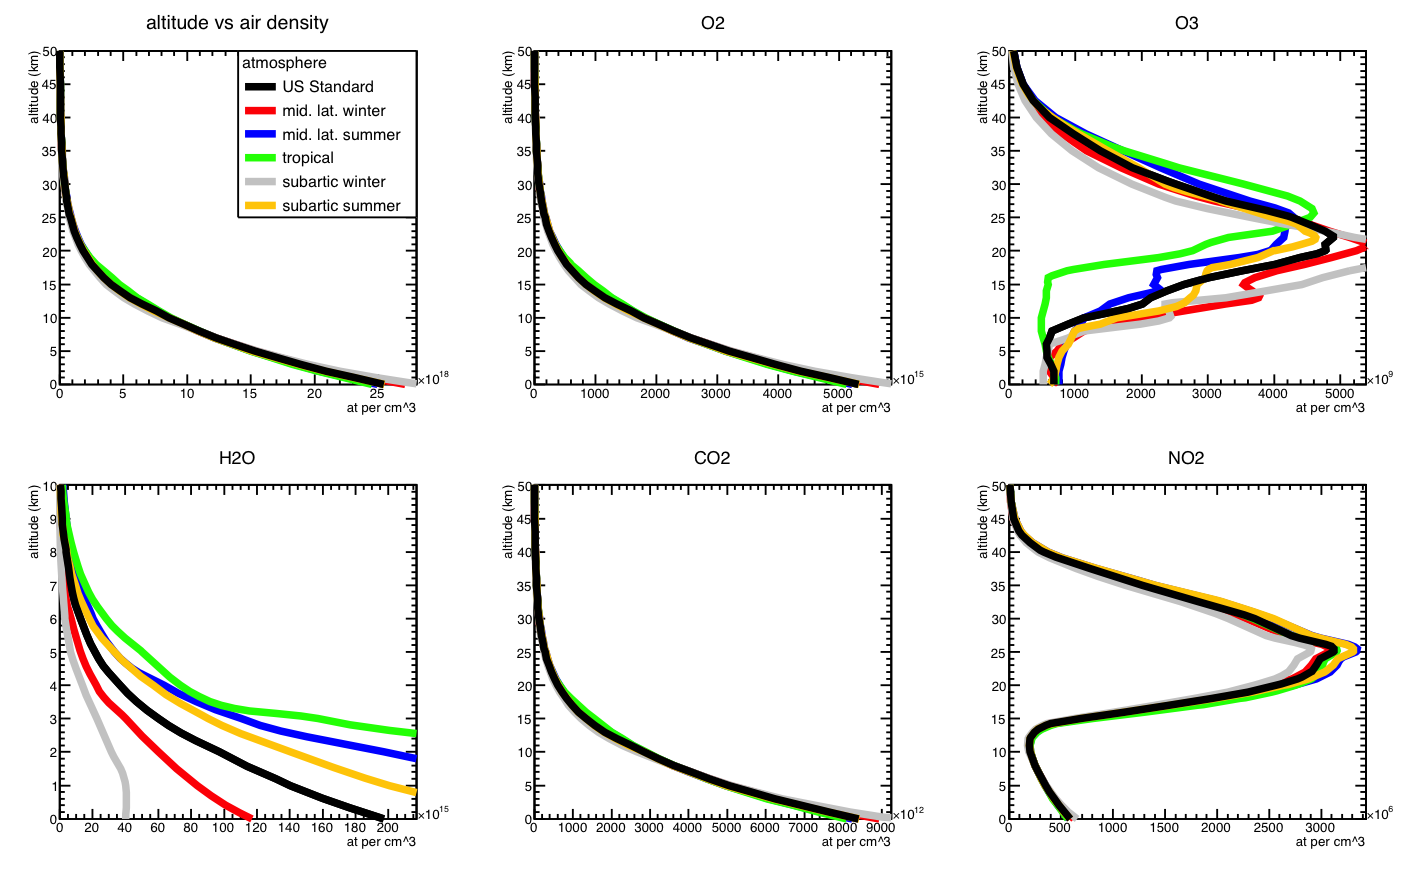
\includegraphics[width=1\textwidth]{images/rt_atm_densities.png}
\caption{\label{fig:rt_atm_densities}Densities profiles for different molecules in air for typical atmospheres in LibRadtran.}
\end{figure}

Thus we propose to use the two standard atmospheres (AFGL-TR-86-0110~\cite{AFGL76}, which are probably both defined in Modtran and LibRadtran, 
the standard US atmosphere and also the subarctic winter the driest  climate which may be well suited to LSST. 
\atmosconfig[inline]{ {\bf Atmospheric models :} AFGL atmospheric constituent profile~: U.S. standard atmosphere 1976 and Subarctic Winter.}
 
 
The US atmosphere is shown as the black line in figure~\ref{fig:rt_atmprof} and ~\ref{fig:rt_atm_densities}. 
This US atmosphere is a good choice because it is not a extreme case. 
Really it can be considered as an average of all other atmospheric models. It shows an average PWV at ground and also an average Temperature at the  20-25~km altitude.

\section{Comparison of Rayleigh Scattering}
%-------------------------------------------------------

Rayleigh scattering is also called molecular scattering. It is an elastic scattering of light on the molecules of the atmosphere. 
The proposition is to simulate a pure Rayleigh atmosphere by switching off any other scattering process like the particle or Mie scattering also called the Aerosols scattering.

The Figure~\ref{fig:rt_rayleigh} hows the air transparencies obtained by LibRadtran for the 10 selected air-masses.
\begin{figure}
\centering
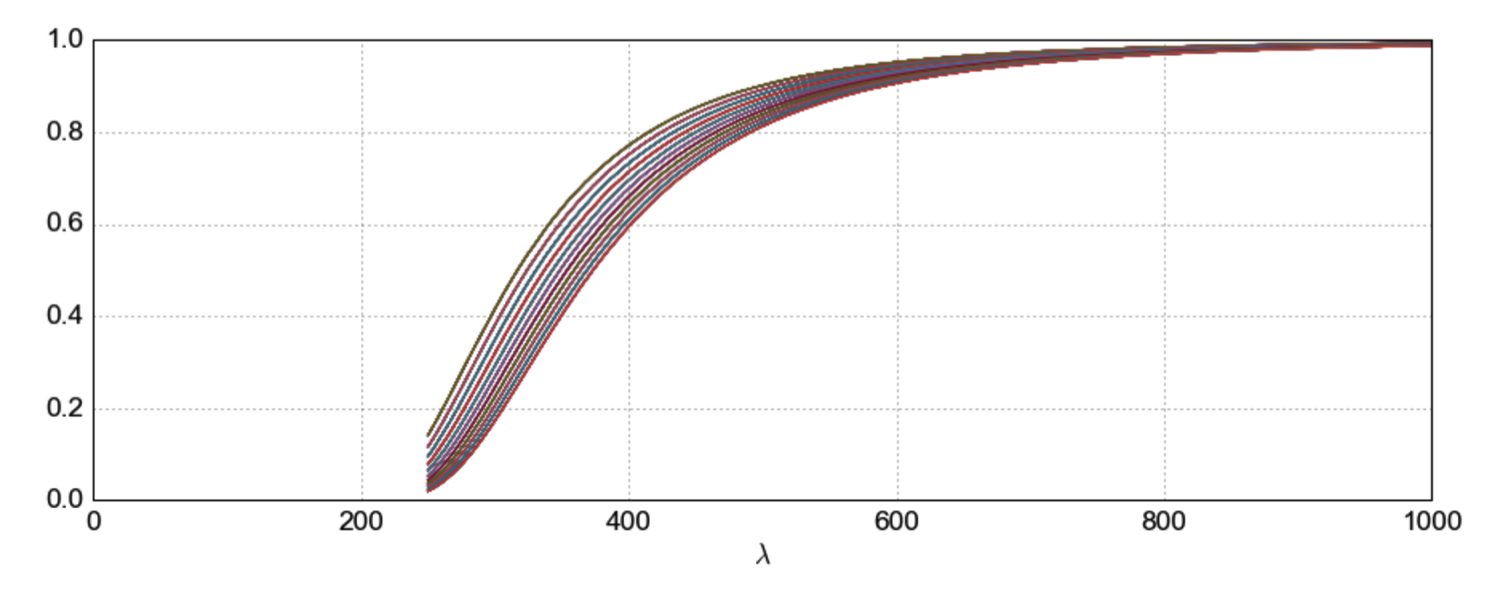
\includegraphics[width=\textwidth]{images/rt_rayleigh}
\caption{\label{fig:rt_rayleigh}Air transparencies attenuation predicted by LibRadtran for US standard atmosphere, when only Rayleigh scattering is selected and all other processes like aerosols scattering and molecular absorption are switched off. The different lines are obtained by varying the airmass $z=1.,1.1,1.2,1.3,1.4,1.5,1.6,1.7,1.8,1.9,2.0$.}
\end{figure}

The comparison of Rayleigh Scattering in Modtran and LibRadtran is not difficult. Indeed, the air optical index $\tau$ can be easily approximated by two formula as follow~\

\begin{equation}
\left\{
\begin{array} {c c c}
\tau& =& \frac{X_v(h)\cdot z}{2770 g/cm^2 } \left( \frac{400 nm}{\lambda}\right)^4 \\
\tau& =& \frac{X_v(h)\cdot z}{3102 g/cm^2 } \left( \frac{400 nm}{\lambda}\right)^4  \frac{1}{ 1-0.0722\left(\frac{400nm}{\lambda}\right)^2} 
\end{array}
\right.
\label{eq:rayleighod}
\end{equation}
where is $X-v(h)$ is the atmospheric column depth at altitude $h$ expressed in unit g/cm$^2$ and $z$ is the airmass.
The air transparency is given by $T=e^{-\tau}$.

In our case, we have to choose $h$ as the LSST altitude.

By fitting the simulated air transmittance curve as a function of the wavelength $\lambda$, 
\begin{equation}
\ln T(\lambda)=-\tau(\lambda)=- \frac{C\cdot z}{\left( \frac{400 nm}{\lambda}\right)^4} 
\end{equation}
one can compare the fitted value of the $C$ parameter derived from Modtran and LibRadtran for each of the 10 airmass values $z$.
$C$ should depend only on air density or pressure at altitude $h$.
Thus $C$ values are expected to be very similar within the computer errors.

\molscatprocess[inline]{{\bf Pure molecular scattering~:} Simulate a pure molecular scattering atmosphere for pre-selected airmass and climate, without absorbing component and without aerosols.}

\section{Comparison of Absorption predictions}
%------------------------------------------------------------

We want to compare atmospheric absorption prediction by switching off any scattering process.
An example of such prediction for each of the 10 airmass values $z$ is shown on figure~\ref{fig:rt_absorption}.

\begin{figure}
\centering
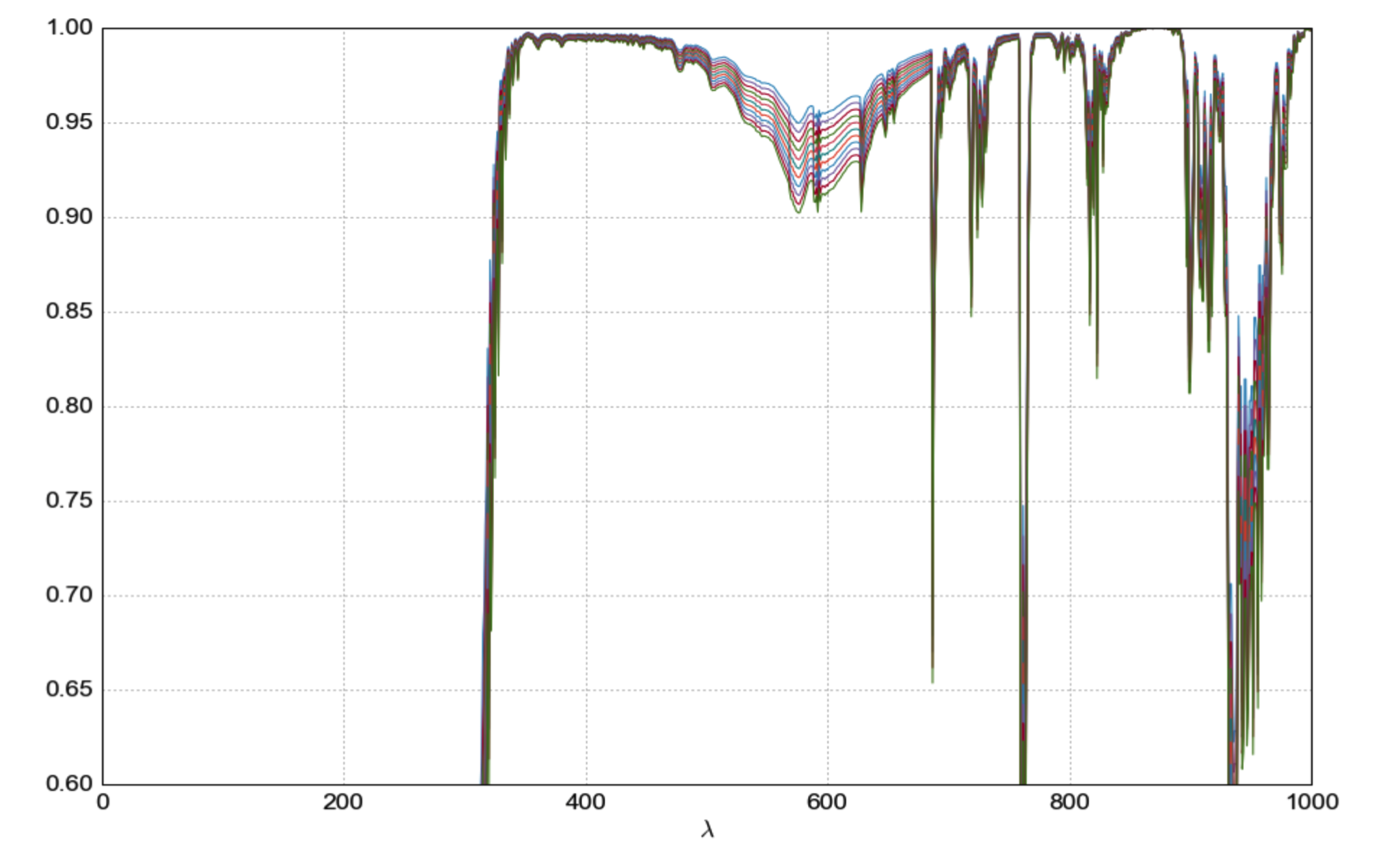
\includegraphics[width=1\textwidth]{images/rt_absorption.png}
\caption{\label{fig:rt_absorption} Air transparency predicted by LibRadtran, when only molecular absorption is selected.}
\end{figure}
Several molecular species in the air show either few strong absorption lines like $O_2$ or wide absorption bands like $H_2O$ (PWV) or $O_3$.

\subsection{Various Absorption Models}
Because bands consist in tens of thousand lines that may overlap, it is usually impossible to compute the absorption line by line.
Instead one has to select different kinds of models which implement absorption in the bands.
These models are probably implemented both in Modtran an LibRadtran as well. However, those models implementation need to be compared.

In the LibRadtran documentation, such models are referred as~:
\begin{itemize}
\item {\bf Spectrally resolved  calculation},
\item {\bf Line-by-line calculation},
\item {\bf The correlated-k method},(Kato and Kato2),
\item {\bf Representative wavelengths parameterization (REPTRAN)},
\item {\bf Pseudo-spectral calculation adapted from LOWTRAN}. 
\end{itemize} 

Probably, there is no need for perfectly well resolved lines calculations (which consumes much simulation time) for LSST broad band photometric measurements.
We suggest to simulate only the "correlated-k method", the "Representative wavelengths parameterization" and the "Pseudo-spectral calculation".

\molabsmodel[inline]{{\bf Absorption models~:} 1) REPTRAN, 2) LOWTRAN, 3) KATO2, 4) KATO}


\subsection{Variable component specifications}


Once the absorption models, one has to specify the amount of variable components in the selected atmosphere.
The two variable molecular component of interest for LSST are the precipitable water vapor (PWV) and Ozone ($O_3$).
Even if the standard atmosphere include a default value for such component, we strongly recommend to overwrite the standard value by a set of pre-defined values.


\subsubsection{Precipitable Water Vapour}
%-------------------------------------------------


We can vary the $H_2O$ pwv in a wide range of values as shown on figure~\ref{ig:ew}.
\begin{figure}
\centering
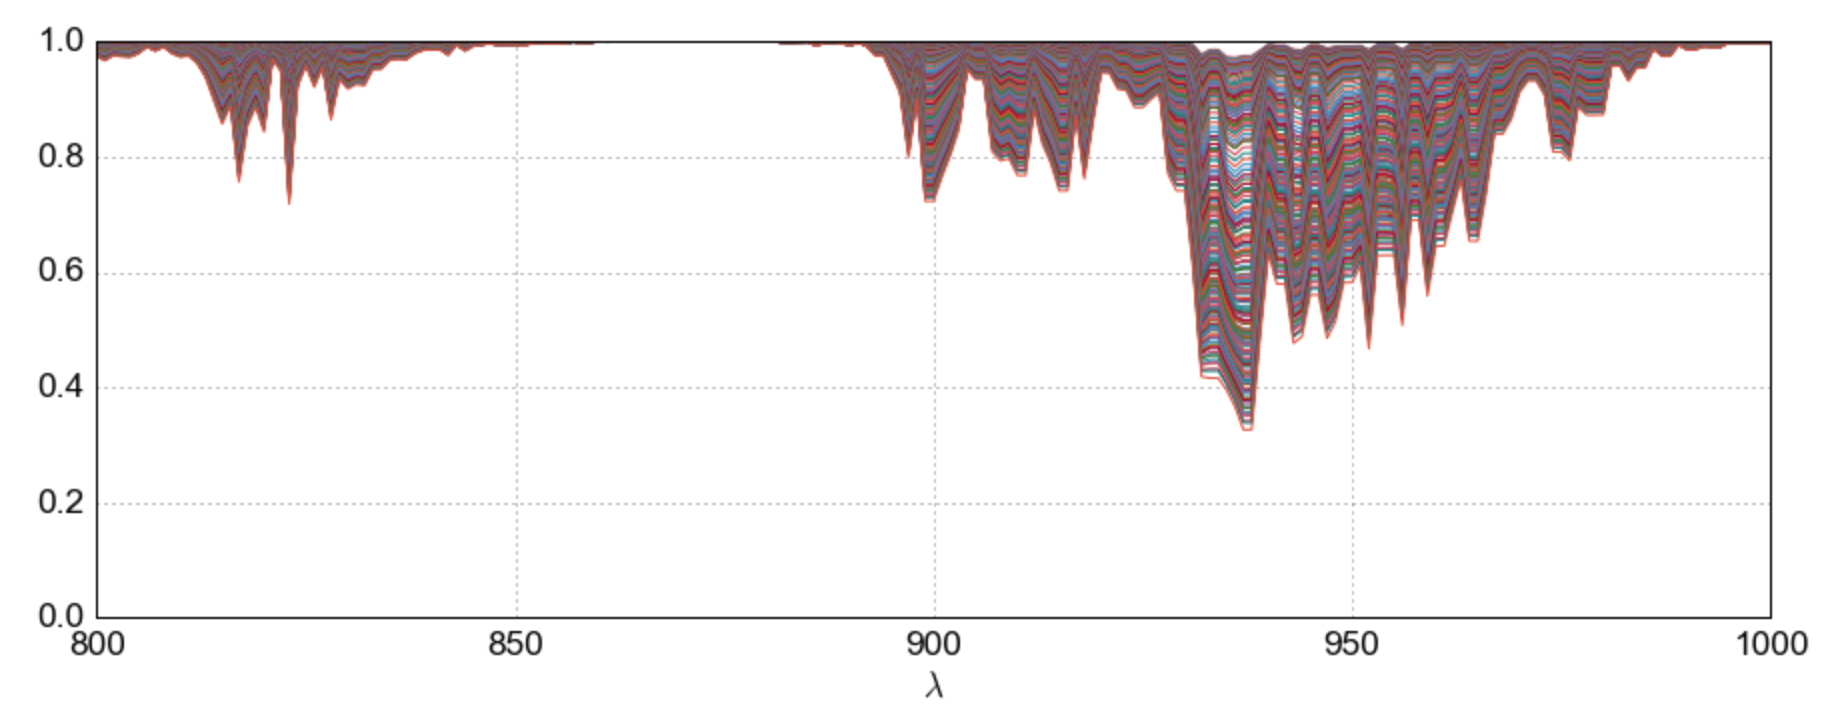
\includegraphics[width=0.8\textwidth]{images/pwv}
\caption{\label{fig:ew}Simulation of absorption by PWV for PWV ranging from $0.1, 0.2,0.3, \cdots 9,8,9.910$~mm.}
\end{figure}

\molabscompo[inline]{ {\bf $H_2O$ PWV : }Generate Modtran/LibRadtran absorption profiles  for 31 points $pwv$ $\in \left[0~{\rm mm},15~{\rm mm} \right]$ in steps of 0.5~mm (and fix $O_3$ to 300 Dobson unit).}



\subsubsection{Ozone}
%----------------------------

Again we can vary the amount of Ozone in the atmosphere we have selected~:
\molabscompo[inline]{ {\bf $O_3$ absorption bands} : Generate Modtran/LibRadtran absorption profiles in grids of 21 points $O_3$ $\in \left[200~{\rm Dobson},600~{\rm Dobson} \right]$ (and fix pwv to 3~mm).}


\section{Combination of scattering and absorption}
%----------------------------------------------------------------
We have to combine the molecular scattering process with the molecular absorption processes.

\allruns[inline]{{\bf Combined light interaction processes~:} simulate pure molecular scattering, pure molecular absorption, combined molecular scattering and absorption.}


\section{Comparison of Aerosols}
%------------------------------------------
The simulation of aerosols may be done by specifying the Aerosol Optical Depth (AOD) $\tau_0$ at a given wavelength $\lambda_0$ and giving the value of the Angstrom exponent $\alpha$ such the effective optical depth $\tau_{aer}(\lambda)$ is~:
\begin{equation}
\tau_{aer}(\lambda)= \tau_0 \cdot \left( \frac{\lambda_0}{\lambda}\right)^\alpha
\end{equation}

\aerosols[inline]{{\bf Aerosols~:}  $\tau_0 \in [0, 0.5]$ in steps of 0.01,  $\alpha \in [0,4]$ in steps of 0.5, $\lambda_0=532$~nm. We suggest to simulate this with a pure molecular scattering atmosphere.}

\section{Summary}
%------------------------
\subsection{Summary with color conventions}
The list of the settings for the simulations are listed below~:
\listoftodos[Simulation parameters summary and analysis to compare Modtran and LibRadtran.]

\subsection{Numbers of runs and files}
%-----------------------------------------------

\begin{table}[h]
{\small
\begin{tabular} {|l|l|r|c|r|l|}  \hline\hline
Number of & Variable name & Number & Range & Step & Comment \\ \hline\hline
Airmass    &   $z$                 &     31     & $[1,3]$ & 0.1   & Check PP wrt PS \\
Solvers     & $rte$             &       2      & $(PP,PS)$ &    &  Radiative transfer Eq. \\
Atmosphere &  $atm$       &     2        &  $(us,sw)$ &   &  out of 6 standards def.\\
Light inter. procs    &  $procs$    &   4          & $(mol\_scatt,mol\_abs,mol\_all)$ & & no aerosols \\
Abs Models  & $amod$  & 4 & $(rept,lowt,kato2,kato)$ & &  \\
Water vapor  & $pwv$    & 31 & $[0,15]$ & 0.5  & $O_3$ set to 300 Dobson \\
Ozone        & $O_3$      & 21  & $[200,600]$ & 20 & $pwv$ set to 3~mm \\ \hline
Aerosols1     &  $\tau_0$  & 51  & $[0,0.5]$   & 0.01 &  \\
Aerosols2     & $\alpha$  &  17 & $[0,4]$ & 0.25 &  \\ \hline 
\hline
\end{tabular}
}
\end{table}

\subsection{Counting the files}

\subsubsection{Pure molecular scattering files (Rayleigh)}
%---------------------------------------------------------------------------

\begin{eqnarray}
N^{files}_{molscat} & = & N_z \times N_{rte} \times N_{atm} \\ \nonumber
                               & = & 31 \times 2 \times 2  = 124
\end{eqnarray}

\subsubsection{Pure molecular absorption files}
%----------------------------------------------------------------

The number of pure molecular absorption files with varying $H2_0$~:

\begin{eqnarray}
N^{files}_{molabs}(H_2O) & = & N_z \times N_{rte} \times N_{atm} \times N_{proc} \times N_{amod} \times N_{pwv} \\ \nonumber
                                          & =  & 31   \times   2        \times    2         \times     4        \times     4            \times 31 = 61504
\end{eqnarray}

The number of pure molecular absorption files with varying $O_3$~:

\begin{eqnarray}
N^{files}_{molabs}(O_3) & = & N_z \times N_{rte} \times N_{atm} \times N_{proc} \times N_{amod} \times N_{O3} \\ \nonumber
                                          & =  & 31   \times   2        \times    2         \times     4        \times     4            \times 21 = 41664
\end{eqnarray}



\subsubsection{Combined molecular scattering and absorption}
%------------------------------------------------------------------------------------

In this case we double the number of files we had to simulate for pure molecular absorption.
Thus we would have another 103168 files.

In total we would generate 206460 files.


\subsubsection{Variation of aerosols}
For the aerosols, we assure to use a single configuration of molecular scattering and absorption.
We have to simulate aerosols over a two parameter grid~:
\begin{eqnarray}
N^{files}_{molabs}(H_2O) & = & N_z \times N_{rte} \times N_{atm} \times N_{\tau} \times N_{alpha}  \\ \nonumber
                                          & =  & 31   \times   2        \times    2         \times     31        \times     21            \times 31 = 80724
\end{eqnarray}




\subsubsection{File size and total file size}
%-------------------------------------------------------
For LibRadtran, the output is a file of two columns. First column is the wavelength. The second column is the air transmittance.
In total, there are 1101 lines.

The typical file size is 25kB.

\begin{itemize}
\item We need at least 5.2  GB storage, without aerosols. 
\item If we want to simulate an aerosols grid, we would need at least 2~GB.
\end{itemize}

\section{File naming conventions}
%-----------------------------------------

We can propose a file naming convention accounting for the selected parameters for the simulation~:
\begin{equation}
{\rm  P\_O\_\{rte\}\_\{atm\}\_\{proc\}\_\{mod\}\_zXX\_wvXX\_ozXX.extension  }\nonumber
\end{equation}

\begin{itemize}
\item [{\bf P :} ] {\bf RT} or {\bf MT} for LibRadtran or Modtran,
\item [{\bf O :} ]  Observatory site {\bf LS} or {\bf HP}  or {\bf GM}  or {\bf MK} for LSST, OHP, Gemini South, Mauna Kea,...
\item [{\bf \{rte\} :}] {\bf pp} or  {\bf ps},
\item [{\bf \{atm\} :}]  {\bf us} or {\bf sw},
\item [{\bf \{proc\} :}] {\bf sc} for pure molecular scattering, {\bf ab} for pure molecular absorption, {\bf sa} for the combination of molecular scattering and absorption,
\item [{\bf \{mod\} :}] {\bf rt} for Reptran model, {\bf lt} for Lowtran model, {\bf k2} for Kato2 model, and {\bf kt} for Kato model.
\item [{\bf zXX :} ] Airmass $z$, where XX is the value of the airmass on 2 digit $XX=2\times z$,
\item [{\bf wvXX :} ] Precipitable water vapour $pwv$, where XX is the value of the $pwv$ on 3 digit $XXX=10\times pwv$, $pwv$ in mm unit,
\item [{\bf ozXX :} ] Ozone $oz$, where XX is the value of the $oz$ on 2 digit $XX=oz/10$, $oz$ is Dobson unit.
\end{itemize}

File extension may be chosen to be $extension=dat$ or $extension=txt$.

For example a filename for LibRadtran, for LSST could be~:
\begin{equation}
RT\_LS\_pp\_us\_sa\_rt\_z15\_wv030\_oz30.txt  \nonumber
\end{equation}
where $pwv=3$~mm and $oz=300$~Dobson unit and $z=1.5$.


\section{Files organisation}
%-----------------------------------------
We may suggest a hierarchical structure  of the files in embedded directories.
Each leaf directory provides the set of simulated files of varying $z$ and $pwv$ or $oz$ in case of molecular absorption, for a given atmospheric and absorption model configuration.

\begin{table}[h]
{\small
\begin{tabular}{ l l}
  rootdir &  top directory \\
 rootdir/RT/VXX/LS/pp/us/sc/ & pure molecular scattering \\
 rootdir/RT/VXX/LS/pp/us/ab/rep/pwv/ & pure molecular absorption for varying $pwv$ \\
 rootdir/RT/VXX/LS/pp/us/ab/rep/oz/ & pure molecular absorption for varying $oz$ \\
 rootdir/RT/VXX/LS/pp/us/sa/rep/pwv/ & molecular absorption and scattering for varying $pwv$ \\
 rootdir/RT/VXX/LS/pp/us/sa/rep/oz/ & molecular absorption scattering for varying $oz$ \\
 rootdir/RT/VXX/LS/pp/us/sc/ae/ & pure molecular scattering and aerosols scattering \\
 rootdir/RT/VXX/LS/pp/us/sa/rep/ae/ & molecular absorption scattering and aerosols scattering \\
\end{tabular}
}
\end{table}
$VXX$ is the version number of Radtrran or Modtran.

In a leaf directory, interpolation of spectra in $z$ and either $pwv$ or $oz$ is possible.


\newpage
\appendix

%----------------------------------------- Not to be shown ----------------------------------------------------------------------------------
\thiswillnotshow[inline]
{ 
\section{Analytical models for Absorption}
A question can be raised~: is it possible to parameterize the transmittance of absorption lines.
Theoretically yes. Absorption can be parameterized by the absorption coefficient $k_\nu$ where $\nu=hc/\lambda$~:
\begin{equation}
k_\nu=S(T) f(\nu-\nu_0)
\end{equation}
$S(T)$ is the energy level transition strength, depending only on temperature according a known analytic formula derived by  quantum mechanics.
$f(\nu-\nu_0)$ is the normalised absorption line shape, which resonant frequency is $\nu_0$, with a natural width $\alpha(P,T)=\alpha_0 \frac{P}{P_0}\left( \frac{T_0}{T}\right)^n$.
$\alpha_0$ is the half reference width for STP ($T_0=273$~K, $P=1013$~mb).
For most gazes, the exponent $n=1/2$.
The analytical formula for the shape $f(\nu-\nu_0)$ is also known.
It is a Lorenzian in the troposphere, where the dominant absorption line broadening is due to molecules collisions.
All the parameters $S(T)$, $\alpha_0$, $n$ for each species are maintained in the spectroscopic database HITRAN~\cite{HITRAN}.


The air transmittance for absorption  $T_\nu(u)$ and the absorbance $A_\nu(u)=1-T_\nu(u)$  are calculated from $k_\nu$\footnote{These formula are given for $k_\nu(u)$ constant along the path length $u$. If $k_\nu(u)$ is not constant, then one can replace  $k_\nu \cdot u  = \int_u  k_\nu(u^\prime) du^\prime$. }~:

\begin{equation}
\left\{
\begin{array}{ccl}
T_\nu(u) & = & e^{  - k_\nu \cdot u } \\
A_\nu(u) & = & \frac{1}{\Delta \nu} \int_{\Delta \nu} ( 1 - e^{  - k_\nu \cdot u} )d\nu
\end{array}
\right.
\end{equation}

where $u$, the path length for an absorber with density $\rho_a$ is given by~:
\begin{equation}
u = \int_0^z \rho_a(z^\prime)dz^\prime
\end{equation}

If we define the equivalent width $W$ for a single absorption line such $W=A_\nu \Delta \nu$, then the equivalent width can be calculated as follow\footnote{$L(x)= x e^{-x}(I_0(x)+I_1(x)) $ is the Ladenburg and Reiche function. $L(x)\approx x\left( (1+(\frac{\pi x}{2})^{5/4}\right)^{-2/5}$. For small $x$, $L(x)\approx x$. For large $x$, $L(x)\approx \left( \frac{2x}{\pi}\right)^{1/2}$.}~:
\begin{equation}
W = 2\pi \alpha L(x)=2\pi \alpha x e^{-x}(I_0(x)+I_1(x))
\end{equation}
where~:

\begin{equation}
 x=\frac{Su}{2\pi\alpha}
\end{equation}

The equivalent width can be easily calculated from the absorption curve as shown on figure~\ref{fig:ew}

\begin{figure}
\centering
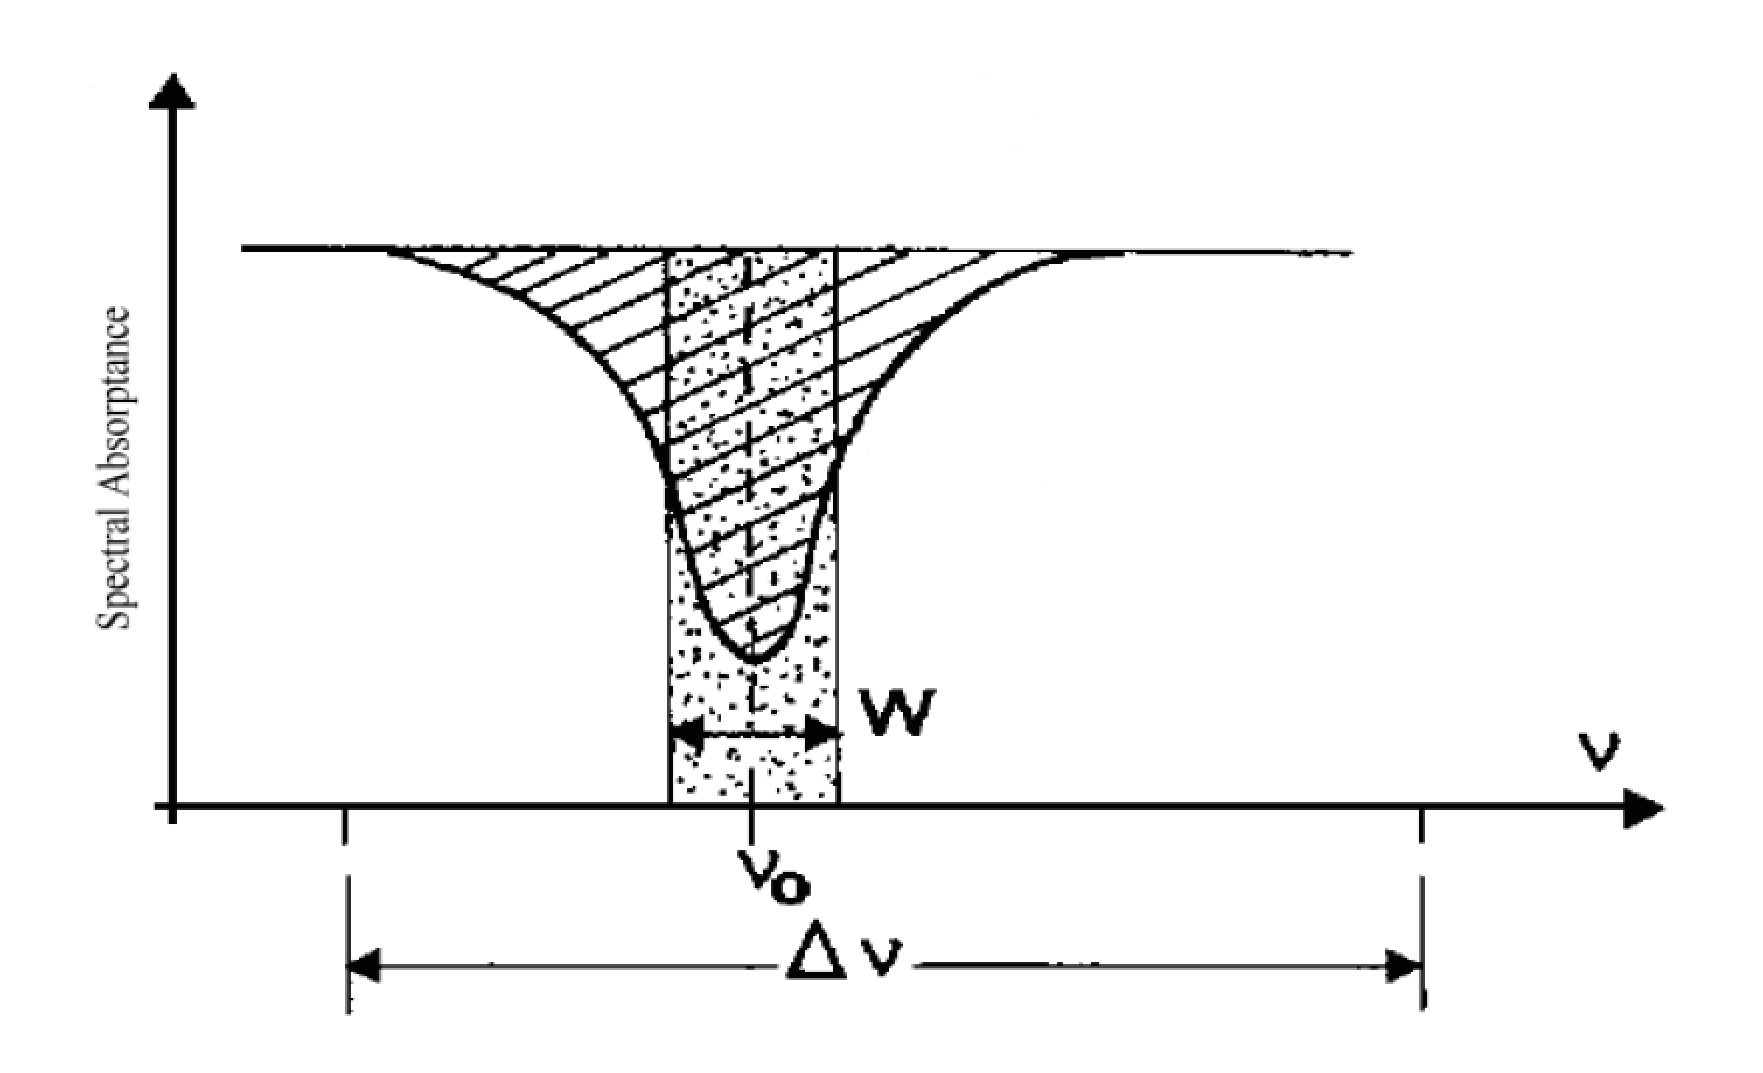
\includegraphics[width=0.8\textwidth]{images/ew}
\caption{\label{fig:ew}Concept of equivalent width.}
\end{figure}


The equivalent width can be parameterised very simply under the assumptions of weak absorption $ x<<1$ and strong absorption $x>>1$~:

\begin{equation}
\fbox{$
\left\{
\begin{array}{ccl r}
W & = & S\cdot u  \propto z  & ({\rm no \; saturation\; }x<<1)\\
W & = & 2\sqrt{\alpha \cdot S\cdot u}  \propto \sqrt{z}  & ({\rm strong\;saturation\;} x>>1)\\
\end{array}
\right.
$}
\label{eq:ew}
\end{equation}

where $z$ is the airmass.


Precipitable water vapour absorptions consist in many lines grouped in bands. We can still use the concept of equivalent with. However we cannot use the single line
formula given in equation~\ref{eq:ew}.
Nevertheless several formula can be derived~:

\subsection{Oxygen}
%----------------------------
The fraction of oxygen in the air is 21\% of the molecules. Because of the large number of oxygen molecules in air  and the strong absorption line $S_{O2}(T)\cdot u >>1$. Thus the line is strongly saturated.

 
%\todo[inline]{$O_2$ absorption line :  Compare in $W$ vs $z$ in Modtran/LibRadtran, and make a fit of a function $W(\beta,\gamma) = \gamma\cdot L(\beta z)$.}
%In addition, we should be able to compare Modtran/LibRadtran prediction to Hitran absorption prediction for $W$ assuming most of the $O_2$ molecules are located at an altitude $h=h_{LSST}$ at a temperature $T(h_{LSST})$.



\subsubsection{Statistical Goody band model}
%-----------------------------------------------------

\begin{equation}
\fbox{$
T_\nu=\exp\left( - \frac{\overline{S}u}{\delta}\left( 1+\frac{\overline{S}u}{\pi \alpha} \right)^{-1/2} \right)
$}
\end{equation}
where $\frac{\overline{S}}{\delta}$ and $\frac{\overline{S}}{\pi \alpha}$ are parameters to fit.

\subsubsection{Malkus band model}
%---------------------------------------------------

\begin{equation}
\fbox{$
T_\nu=\exp \left(
 - \frac{\pi \alpha}{2\delta}\left( \left(1+\frac{4\overline{S}u}{\pi \alpha} \right)^{1/2}  -1\right)
 \right)
$}
\end{equation}

\paragraph{Weak line limit : $\frac{\overline{S}u}{\pi \alpha}<<1$~:}

\begin{equation}
\fbox{$
T_\nu=\exp \left(
 - \frac{\overline{S}u}{\delta}
 \right)
$}
\end{equation}


\paragraph{Strong line limit : $\frac{\overline{S}u}{\pi \alpha}>>1$~:}
\begin{equation}
\fbox{$
T_\nu=\exp \left(
 - \frac{\sqrt{\pi\alpha \overline{S}u}}{\delta}
 \right)
$}
\end{equation}

%-------------------------------------------------------------------------------------------------------------------------------------
}  % not to be shown

\newpage

\appendix

\section{Minutes}

\begin{verbatim}
Kirk, Sylvie et al, 

Below are short minutes of our Friday meeting.  I think we had a
productive discussion, thank you all for your time.  I try to be
short. Please email me if you think I have forgotten something.

Atmosphere models : MODTRAN / libRadTran comparison
====================================================

 (*) Sylvie is finishing up a note, where she discusses input parameters
     for libRadtran. The goal is to define a standard atmosphere, not
     too different from what we have at Cerro Pachon, and to generate a
     grid of libRadTran models around this standard atmosphere. 

 (*) Regarding the atmosphere profiles: there are several standard
     options available in libRadTran (and MODTRAN).  For the moment,
     Sylvie is going to pick "US standard" and "Arctic Winter" and
     generate the same grid of model for each of these profiles.

 (*) Sylvie has not yet explored the aerosols options (in particular,
     everything regarding the typical particle sizes) in detail. The
     atmosphere models will have an aerosol component, which may require
     further refinements in the future.

 (*) Sylvie will produce the transmission curves of the individual
     components alongside her full models. 

 (*) Kirk is going to generate the same grid of models, (same
     parameters, same assumptions, same atmosphere profiles) with
     MODTRAN.

 (*) These grids of models will be uploaded on the github repository of
     Key Task #5 (atmospheric models).  Sylvie and Kirk have code too,
     that will be uploaded there.

 (*) in a second step, similar grids will be produced for an atmosphere
     that is typical of OHP.


Modeling the telescope <-> stardice line of sight at OHP
========================================================

 (*) Kirk is going to produce a grid of atmospheric transmissions for
     the configuration we have at OHP : horizontal line of sight,
     L=250-m, pressure, PWV, Ozone, aerosol opt. depth to be transmitted
     by Sebastien.


Preliminary model comparisons
=============================

 (*) The first step, when comparing libRadtrans vs.  MODTRAN
     transmission, is to determine, for any given transmission generated
     with one model, how well (and for what value of its parameters) the
     other can reproduce this transmission.

 (*) Sylvie has sent models typical of the atmosphere at OHP to
     Sebastien, who has performed a preliminary comparison with the
     Buton et al model (tuned on observations performed at Mauna Kea)

 (*) Sebastien has shown that the Buton model can reproduce the
     transmissions sent by Sylvie well. 

CTIO spectroscopic data
=======================

 (*) Kirk presents the data he has taken at CTIO. These are
     spectroscopic observation of (CALSPEC?) stars, followed 
     during the night, over a wide range of airmass.

 (*) an interesting goal is to explore whether one can describe the
     variations of atmospheric absorption with MODTRAN.

 (*) Kirk is going to produce a data release (files + models + current
     version of his fit code + readme)

TODO:
=====

 (*) Nicolas creates a git repository for Key Task #5

 (*) Sylvie and Kirk generate grids of libRadTran and MODTRAN models
     around a typical Cerro Pachon atmosphere.

 (*) In a second step, they produce similar grid for a typical
     atmosphere at OHP and Mauna Kea.

 (*) Kirk produces a grid of model for the horizontal line of sight at
     OHP.

 (*) Kirk prepares a data release for the CTIO / Pachon data.

Nicolas.
\end{verbatim}

\section*{Github}
\begin{verbatim}
Dear all, 

Just letting you know that I have created a new git repository for the
PCWG work on the atmospheric extinction. 

It is here:

https://github.com/DarkEnergyScienceCollaboration/PC5AtmosphericExtinction

At the moment, the repository is private.  Shall I make it public ?  It
think it can be public. If the consensus is that it should be kept
private, please send me your github usernames, so that I can grant
access to it.

Regards, 

Nicolas.
\end{verbatim}


\begin{thebibliography}{9}

\bibitem{LibRadtran1} 
Technical note : The LibRadtran software package for radiative transfer calculations- description and exemples of use\\
Bernhard Mayer, Arve Kylling\\
Atmos. Chem. Phys. (2005),5, 1855-1877
  
\bibitem{LibRadtran2} 
LibRadtran user's guide\\
Bernhard Mayer, Arve Kylling, Claudia Emde, Robert Buras, Ulrich Hamann, Josef Gasteiger, Bettina Richter \\
Edition for libRadtran version 2.0, Agust 24, 2015

\bibitem{AFGL76} 
AFGL Atmospheric Constituent Profiles (0-120km)\\
G.P. ANDERSON,  J.H. CHETWYND, S.A. CLOUGH, E. P. SHE1TLE, F.X. KNEIZYS \\
AFGL-TR-86-0110\\
\href{http://adsabs.harvard.edu/abs/1986aacp.book.....A}{http://adsabs.harvard.edu/abs/1986aacp.book.....A}

\thiswillnotshow[inline]
{ 
\bibitem{Liou}
Radiation and Cloud Processes in the Atmopshere\\
K.N. Liou \\
1992,Oxford University Press

\bibitem{HITRAN}
The HITRAN Database \\
\href{https://www.cfa.harvard.edu/hitran/}{https://www.cfa.harvard.edu/hitran/}
}
\end{thebibliography}
\end{document}